\begin{figure}[!htbp]
    \centering
    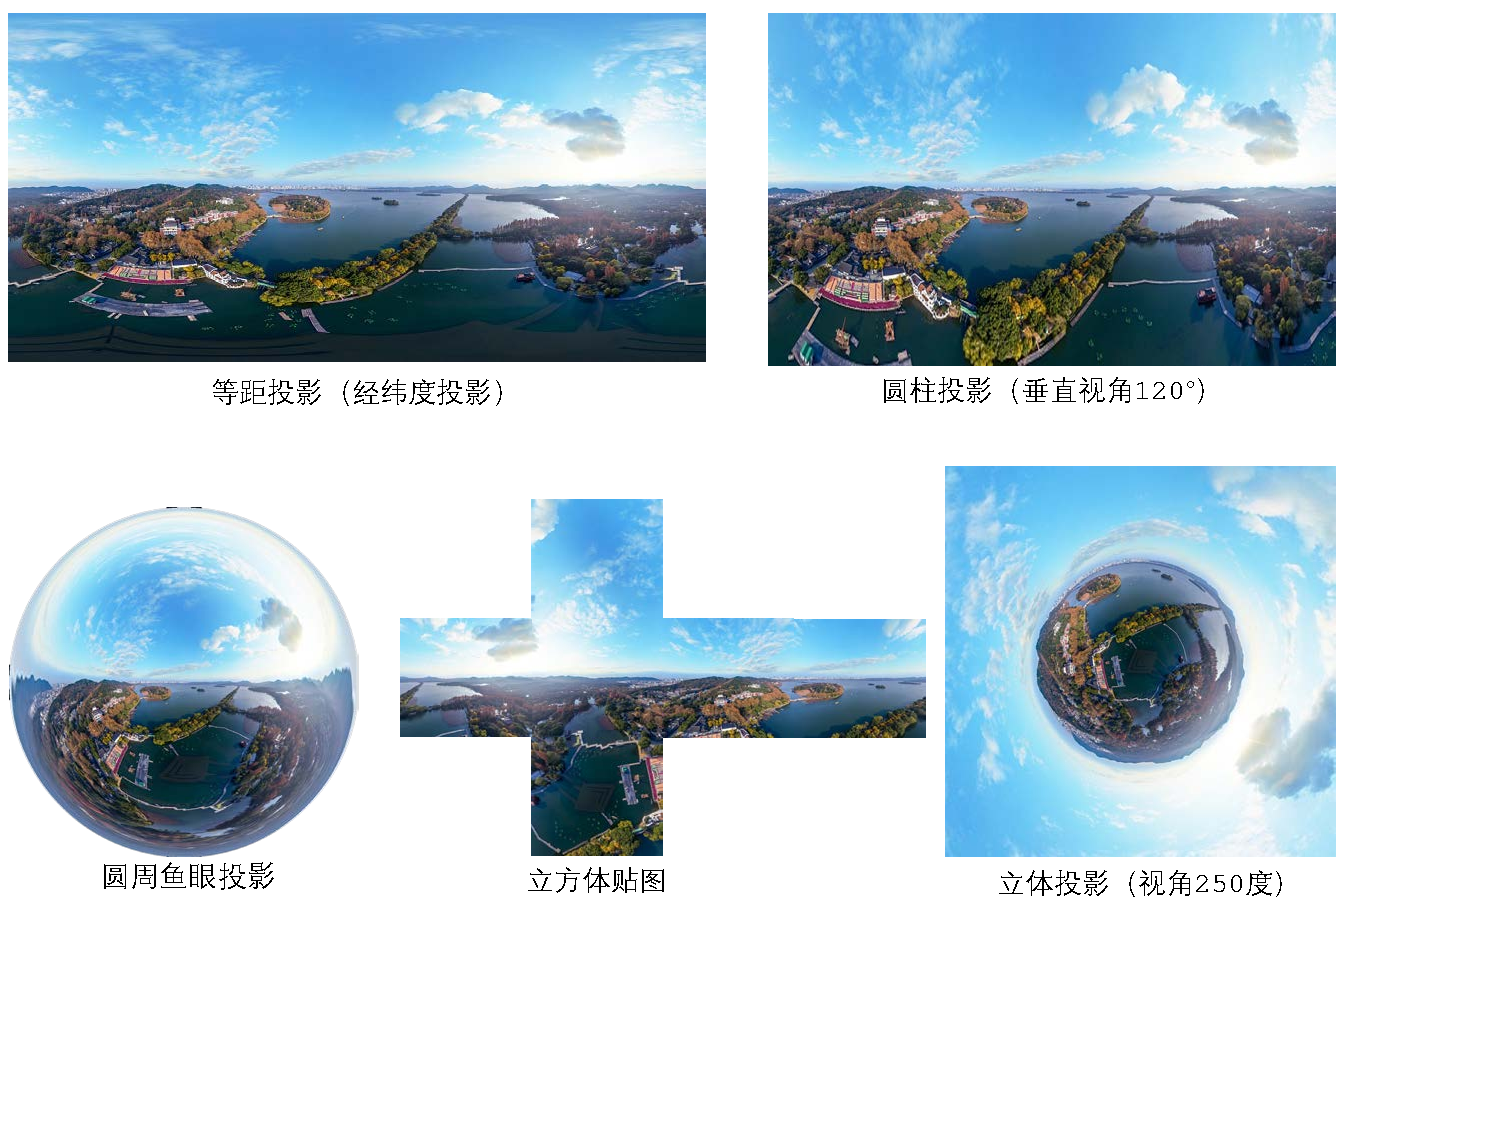
\includegraphics[width=1.0\textwidth]{Img/panorama-projection.pdf}

    \caption[全景图的几种投影方式]
    {
        \label{fig:panorama-projection}
        全景图的几种投影方式。等距投影是常见的全景图投影方式,包括了所有视角的信息。圆柱投影的特点致使它不可能有180\doge的垂直视角;圆周鱼眼投影可以显示出所有视角的信息,但是从中可以看到,靠近圆形边缘的区域被极度扭曲,这会因为计算误差导致精度的损失;立方体贴图是计算机图形学中常用的投影方式;立体投影方式看起来像一颗星球,因此也被成为小行星投影方式,这种方式也无法展示所有视角的信息。
    }
\end{figure}